% Created by tikzDevice version 0.6.2-92-0ad2792 on 2013-02-07 02:00:58
% !TEX encoding = UTF-8 Unicode
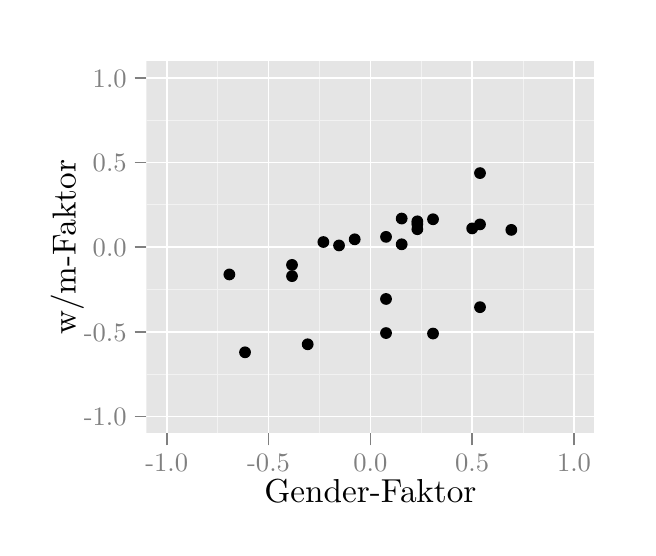
\begin{tikzpicture}[x=1pt,y=1pt]
\definecolor[named]{fillColor}{rgb}{1.00,1.00,1.00}
\path[use as bounding box,fill=fillColor,fill opacity=0.00] (0,0) rectangle (216.81,180.67);
\begin{scope}
\path[clip] (  0.00,  0.00) rectangle (216.81,180.67);
\definecolor[named]{drawColor}{rgb}{1.00,1.00,1.00}
\definecolor[named]{fillColor}{rgb}{1.00,1.00,1.00}

\path[draw=drawColor,line width= 0.6pt,line join=round,line cap=round,fill=fillColor] (  0.00,  0.00) rectangle (216.81,180.68);
\end{scope}
\begin{scope}
\path[clip] ( 42.89, 34.03) rectangle (204.77,168.63);
\definecolor[named]{fillColor}{rgb}{0.90,0.90,0.90}

\path[fill=fillColor] ( 42.89, 34.03) rectangle (204.77,168.63);
\definecolor[named]{drawColor}{rgb}{0.95,0.95,0.95}

\path[draw=drawColor,line width= 0.3pt,line join=round] ( 42.89, 55.45) --
	(204.77, 55.45);

\path[draw=drawColor,line width= 0.3pt,line join=round] ( 42.89, 86.04) --
	(204.77, 86.04);

\path[draw=drawColor,line width= 0.3pt,line join=round] ( 42.89,116.63) --
	(204.77,116.63);

\path[draw=drawColor,line width= 0.3pt,line join=round] ( 42.89,147.22) --
	(204.77,147.22);

\path[draw=drawColor,line width= 0.3pt,line join=round] ( 68.64, 34.03) --
	( 68.64,168.63);

\path[draw=drawColor,line width= 0.3pt,line join=round] (105.43, 34.03) --
	(105.43,168.63);

\path[draw=drawColor,line width= 0.3pt,line join=round] (142.22, 34.03) --
	(142.22,168.63);

\path[draw=drawColor,line width= 0.3pt,line join=round] (179.01, 34.03) --
	(179.01,168.63);
\definecolor[named]{drawColor}{rgb}{1.00,1.00,1.00}

\path[draw=drawColor,line width= 0.6pt,line join=round] ( 42.89, 40.15) --
	(204.77, 40.15);

\path[draw=drawColor,line width= 0.6pt,line join=round] ( 42.89, 70.74) --
	(204.77, 70.74);

\path[draw=drawColor,line width= 0.6pt,line join=round] ( 42.89,101.33) --
	(204.77,101.33);

\path[draw=drawColor,line width= 0.6pt,line join=round] ( 42.89,131.92) --
	(204.77,131.92);

\path[draw=drawColor,line width= 0.6pt,line join=round] ( 42.89,162.51) --
	(204.77,162.51);

\path[draw=drawColor,line width= 0.6pt,line join=round] ( 50.24, 34.03) --
	( 50.24,168.63);

\path[draw=drawColor,line width= 0.6pt,line join=round] ( 87.03, 34.03) --
	( 87.03,168.63);

\path[draw=drawColor,line width= 0.6pt,line join=round] (123.83, 34.03) --
	(123.83,168.63);

\path[draw=drawColor,line width= 0.6pt,line join=round] (160.62, 34.03) --
	(160.62,168.63);

\path[draw=drawColor,line width= 0.6pt,line join=round] (197.41, 34.03) --
	(197.41,168.63);
\definecolor[named]{fillColor}{rgb}{0.00,0.00,0.00}

\path[fill=fillColor] (112.51,101.98) circle (  2.13);

\path[fill=fillColor] (118.17,104.19) circle (  2.13);

\path[fill=fillColor] (129.49,105.08) circle (  2.13);

\path[fill=fillColor] (129.49, 70.32) circle (  2.13);

\path[fill=fillColor] (140.81,107.84) circle (  2.13);

\path[fill=fillColor] (163.45, 79.67) circle (  2.13);

\path[fill=fillColor] ( 78.54, 63.36) circle (  2.13);

\path[fill=fillColor] ( 95.52, 90.89) circle (  2.13);

\path[fill=fillColor] ( 95.52, 94.95) circle (  2.13);

\path[fill=fillColor] (174.77,107.60) circle (  2.13);

\path[fill=fillColor] ( 72.88, 91.49) circle (  2.13);

\path[fill=fillColor] (101.18, 66.26) circle (  2.13);

\path[fill=fillColor] (106.85,103.21) circle (  2.13);

\path[fill=fillColor] (129.49, 82.64) circle (  2.13);

\path[fill=fillColor] (135.15,102.39) circle (  2.13);

\path[fill=fillColor] (135.15,111.70) circle (  2.13);

\path[fill=fillColor] (163.45,128.12) circle (  2.13);

\path[fill=fillColor] (146.47,111.44) circle (  2.13);

\path[fill=fillColor] (140.81,109.67) circle (  2.13);

\path[fill=fillColor] (140.81,110.68) circle (  2.13);

\path[fill=fillColor] (146.47, 70.14) circle (  2.13);

\path[fill=fillColor] (160.62,108.13) circle (  2.13);

\path[fill=fillColor] (163.45,109.58) circle (  2.13);
\end{scope}
\begin{scope}
\path[clip] (  0.00,  0.00) rectangle (216.81,180.67);
\definecolor[named]{drawColor}{rgb}{0.50,0.50,0.50}

\node[text=drawColor,anchor=base east,inner sep=0pt, outer sep=0pt, scale=  0.96] at ( 35.77, 36.85) {-1.0};

\node[text=drawColor,anchor=base east,inner sep=0pt, outer sep=0pt, scale=  0.96] at ( 35.77, 67.44) {-0.5};

\node[text=drawColor,anchor=base east,inner sep=0pt, outer sep=0pt, scale=  0.96] at ( 35.77, 98.03) {0.0};

\node[text=drawColor,anchor=base east,inner sep=0pt, outer sep=0pt, scale=  0.96] at ( 35.77,128.62) {0.5};

\node[text=drawColor,anchor=base east,inner sep=0pt, outer sep=0pt, scale=  0.96] at ( 35.77,159.21) {1.0};
\end{scope}
\begin{scope}
\path[clip] (  0.00,  0.00) rectangle (216.81,180.67);
\definecolor[named]{drawColor}{rgb}{0.50,0.50,0.50}

\path[draw=drawColor,line width= 0.6pt,line join=round] ( 38.62, 40.15) --
	( 42.89, 40.15);

\path[draw=drawColor,line width= 0.6pt,line join=round] ( 38.62, 70.74) --
	( 42.89, 70.74);

\path[draw=drawColor,line width= 0.6pt,line join=round] ( 38.62,101.33) --
	( 42.89,101.33);

\path[draw=drawColor,line width= 0.6pt,line join=round] ( 38.62,131.92) --
	( 42.89,131.92);

\path[draw=drawColor,line width= 0.6pt,line join=round] ( 38.62,162.51) --
	( 42.89,162.51);
\end{scope}
\begin{scope}
\path[clip] (  0.00,  0.00) rectangle (216.81,180.67);
\definecolor[named]{drawColor}{rgb}{0.50,0.50,0.50}

\path[draw=drawColor,line width= 0.6pt,line join=round] ( 50.24, 29.77) --
	( 50.24, 34.03);

\path[draw=drawColor,line width= 0.6pt,line join=round] ( 87.03, 29.77) --
	( 87.03, 34.03);

\path[draw=drawColor,line width= 0.6pt,line join=round] (123.83, 29.77) --
	(123.83, 34.03);

\path[draw=drawColor,line width= 0.6pt,line join=round] (160.62, 29.77) --
	(160.62, 34.03);

\path[draw=drawColor,line width= 0.6pt,line join=round] (197.41, 29.77) --
	(197.41, 34.03);
\end{scope}
\begin{scope}
\path[clip] (  0.00,  0.00) rectangle (216.81,180.67);
\definecolor[named]{drawColor}{rgb}{0.50,0.50,0.50}

\node[text=drawColor,anchor=base,inner sep=0pt, outer sep=0pt, scale=  0.96] at ( 50.24, 20.31) {-1.0};

\node[text=drawColor,anchor=base,inner sep=0pt, outer sep=0pt, scale=  0.96] at ( 87.03, 20.31) {-0.5};

\node[text=drawColor,anchor=base,inner sep=0pt, outer sep=0pt, scale=  0.96] at (123.83, 20.31) {0.0};

\node[text=drawColor,anchor=base,inner sep=0pt, outer sep=0pt, scale=  0.96] at (160.62, 20.31) {0.5};

\node[text=drawColor,anchor=base,inner sep=0pt, outer sep=0pt, scale=  0.96] at (197.41, 20.31) {1.0};
\end{scope}
\begin{scope}
\path[clip] (  0.00,  0.00) rectangle (216.81,180.67);
\definecolor[named]{drawColor}{rgb}{0.00,0.00,0.00}

\node[text=drawColor,anchor=base,inner sep=0pt, outer sep=0pt, scale=  1.20] at (123.83,  9.03) {Gender-Faktor};
\end{scope}
\begin{scope}
\path[clip] (  0.00,  0.00) rectangle (216.81,180.67);
\definecolor[named]{drawColor}{rgb}{0.00,0.00,0.00}

\node[text=drawColor,rotate= 90.00,anchor=base,inner sep=0pt, outer sep=0pt, scale=  1.20] at ( 17.30,101.33) {w/m-Faktor};
\end{scope}
\end{tikzpicture}
